% This file was created with tikzplotlib v0.10.1.
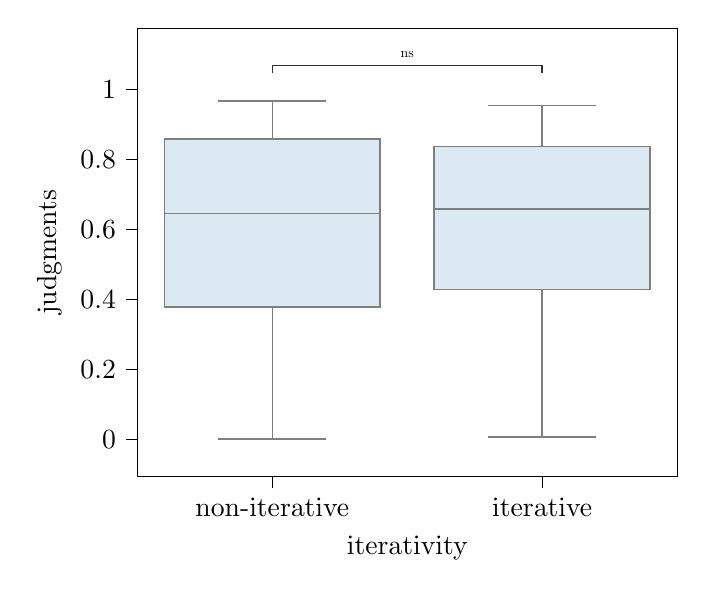
\begin{tikzpicture}

\definecolor{darkgray176}{RGB}{176,176,176}
\definecolor{darkslategray51}{RGB}{51,51,51}
\definecolor{gray127}{RGB}{127,127,127}
% \definecolor{lightgray}{RGB}{211,211,211}
\definecolor{lightgray}{RGB}{219, 234, 242}

\begin{axis}[
tick align=outside,
tick pos=left,
x grid style={darkgray176},
xlabel={iterativity},
xmin=-0.5, xmax=1.5,
xtick style={color=black},
xtick={0,1},
xticklabels={non-iterative,iterative},
y grid style={darkgray176},
ylabel={judgments},
% ymin=-0.0483047604397404, ymax=1.01439996923455,
ytick style={color=black}
]
\path [draw=gray127, fill=lightgray, semithick]
(axis cs:-0.4,0.377803012777129)
--(axis cs:0.4,0.377803012777129)
--(axis cs:0.4,0.85860740650829)
--(axis cs:-0.4,0.85860740650829)
--(axis cs:-0.4,0.377803012777129)
--cycle;
\path [draw=gray127, fill=lightgray, semithick]
(axis cs:0.6,0.427850711243511)
--(axis cs:1.4,0.427850711243511)
--(axis cs:1.4,0.836602473643702)
--(axis cs:0.6,0.836602473643702)
--(axis cs:0.6,0.427850711243511)
--cycle;
\addplot [semithick, gray127]
table {%
0 0.377803012777129
0 0
};
\addplot [semithick, gray127]
table {%
0 0.85860740650829
0 0.966095208794808
};
\addplot [semithick, gray127]
table {%
-0.2 0
0.2 0
};
\addplot [semithick, gray127]
table {%
-0.2 0.966095208794808
0.2 0.966095208794808
};
\addplot [semithick, gray127]
table {%
1 0.427850711243511
1 0.00712199726017315
};
\addplot [semithick, gray127]
table {%
1 0.836602473643702
1 0.953557073154696
};
\addplot [semithick, gray127]
table {%
0.8 0.00712199726017315
1.2 0.00712199726017315
};
\addplot [semithick, gray127]
table {%
0.8 0.953557073154696
1.2 0.953557073154696
};
\addplot [semithick, darkslategray51]
table {%
0 1.04628111112478
0 1.06753520571826
1 1.06753520571826
1 1.04628111112478
};
\addplot [semithick, gray127]
table {%
-0.4 0.644901802592939
0.4 0.644901802592939
};
\addplot [semithick, gray127]
table {%
0.6 0.658667770933208
1.4 0.658667770933208
};
\draw (axis cs:0.5,1.06753520571826) ++(0pt,1pt) node[
  scale=0.5,
  anchor=south,
  text=black,
  rotate=0.0
]{ns};
\end{axis}

\end{tikzpicture}
